\documentclass[11pt]{amsart}
\usepackage{amsmath,amssymb,amsthm}
\usepackage[margin=1.15in]{geometry}
\usepackage{enumitem}
\usepackage{booktabs}
\usepackage{graphicx}
\usepackage[hidelinks]{hyperref}
\usepackage[hypcap=false]{caption}

\newtheorem{theorem}{Theorem}[section]
\newtheorem{lemma}[theorem]{Lemma}
\newtheorem{proposition}[theorem]{Proposition}
\newtheorem{corollary}[theorem]{Corollary}
\newtheorem*{mainA}{Theorem A}
\newtheorem*{mainB}{Theorem B}
\newtheorem*{mainC}{Theorem C}
\newtheorem*{mainD}{Theorem D}
\theoremstyle{definition}
\newtheorem{definition}[theorem]{Definition}
\newtheorem{question}[theorem]{Question}
\theoremstyle{remark}
\newtheorem{remark}[theorem]{Remark}
\newtheorem{example}[theorem]{Example}

\newcommand{\R}{\mathbb{R}}
\newcommand{\C}{\mathbb{C}}
\newcommand{\Z}{\mathbb{Z}}
\newcommand{\MV}{\operatorname{MV}}
\newcommand{\conv}{\operatorname{conv}}
\newcommand{\capn}{\operatorname{cap}}
\newcommand{\miss}{\operatorname{miss}}
\newcommand{\supp}{\operatorname{supp}}
\newcommand{\down}{{\downarrow}}
\newcommand{\SweepX}{10^9}

\numberwithin{equation}{section}

\begin{document}

\title[The extended Courant property, Part I: the square]{The extended Courant property,
Part I:\\ nodal domains of linear combinations of eigenfunctions on the square}

\author{Armaun Sanayei}
\email{arsan{@}alumni.stanford.edu}

\date{\today}

\subjclass[2020]{Primary 35P05; Secondary 14P25, 52B20, 11P21, 58J50}
\keywords{Courant nodal domain theorem, extended Courant property, Courant--Herrmann
conjecture, linear combinations of eigenfunctions, Harnack curve theorem, Newton polygons,
Bernstein--Kushnirenko theorem, lattice points in a disc}

\begin{abstract}
A footnote in Courant--Hilbert claims that any linear combination of the first $n$ Dirichlet
eigenfunctions has at most $n$ nodal domains. This extended Courant property (ECP) is false in
general, and on the square $(0,\pi)^2$ it had only been checked for the first thirteen
eigenvalues. We prove an upper bound $U(\lambda)$ for the number of nodal domains of any
combination of eigenfunctions of the square with eigenvalues at most $\lambda$. The proof writes
the combination as $\sin x\sin y\,P(\cos x,\cos y)$ and bounds the nodal domains of $P$ using
an Euler characteristic formula, Harnack's theorem, the Bernstein--Kushnirenko theorem, and a
new argument about the signs of $P$ at the corners. We show that $U(\lambda)\le\dim E_\lambda$,
which gives the Courant--Herrmann bound, and that ECP holds whenever
$H(\lambda)\ge2r(\lambda)-3$, where $H(\lambda)$ counts lattice segments on the convex hull of
the lattice points in a quarter disc and $r(\lambda)$ is the multiplicity. Using two
independent programs and a theorem of Balog and B\'ar\'any, we conclude that the square has ECP
at every eigenvalue up to $\SweepX$ and at every sufficiently large eigenvalue.
\end{abstract}

\maketitle

\begin{center}
\captionsetup{width=0.7\textwidth,font=small}
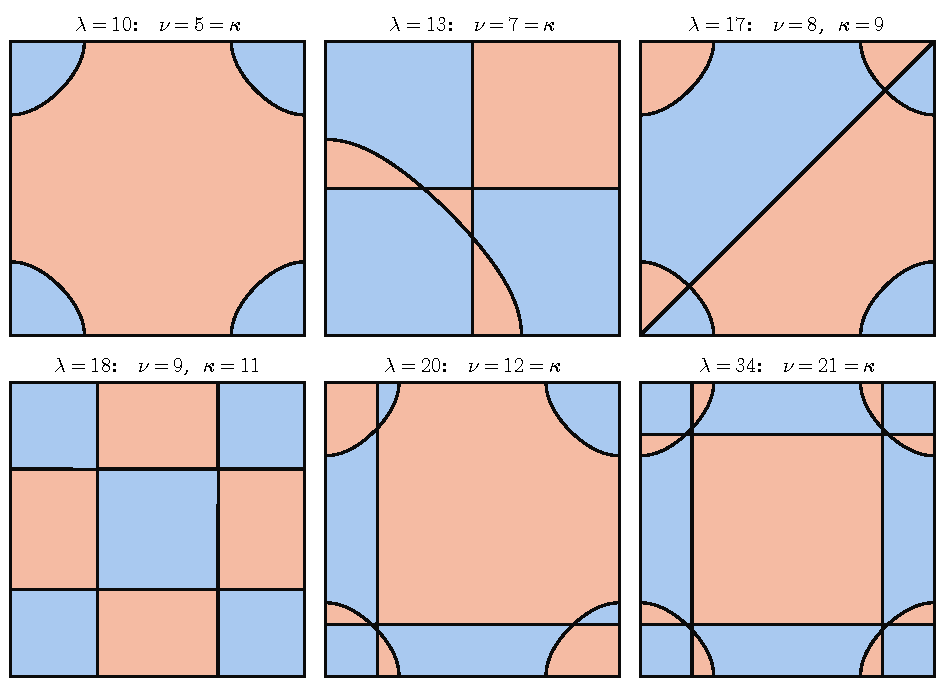
\includegraphics[width=0.66\textwidth]{fig_gallery.pdf}
\captionof{figure}{Combinations of eigenfunctions of $(0,\pi)^2$ with the largest possible
number $\nu$ of nodal domains (blue: positive, orange: negative). At $\lambda=10,13,20,34$
the maximum equals the Courant number $\kappa(\lambda)$; at $\lambda=17$ and $18$ it is smaller
(Propositions~\ref{prop:sharp} and~\ref{prop:17-18}).}
\label{fig:gallery}
\end{center}

%=====================================================================================
\section{Introduction}\label{sec:intro}

Let $\Omega\subset\R^2$ be a bounded domain, with Dirichlet eigenvalues
$\lambda_1<\lambda_2\le\lambda_3\le\cdots$ (counted with multiplicity) and an orthonormal basis
of eigenfunctions $u_1,u_2,\dots$. For a continuous function $f$, we write $\nu(f)$ for the
number of nodal domains of $f$, that is, the number of connected components of $\{f\ne0\}$. In a
1923 paper \cite{Courant23} and in his book with Hilbert \cite{CourantHilbert}, Courant proved
that $\nu(u_n)\le n$. This is Courant's nodal domain theorem.

In a footnote, Courant and Hilbert \cite[p.~454]{CourantHilbert} claim more. They state that any
linear combination $f=\sum_{i\le n}c_iu_i$ also satisfies $\nu(f)\le n$. Following Bérard and
Helffer \cite{BH-I}, we say that $\Omega$ has the \emph{extended Courant property} at $\lambda$
if
\[
\nu(f)\le\kappa(\lambda):=1+\#\{n:\lambda_n<\lambda\}\qquad\text{for all }0\ne f\in
E_\lambda:=\operatorname{span}\{u_n:\lambda_n\le\lambda\}. \tag{ECP$_\lambda$}
\]
Since $\kappa(\lambda_n)\le n$, ECP at every eigenvalue implies the footnote. In fact, ECP at
$\lambda$ is the strongest version of the footnote at that level, since it also covers
combinations that use only part of the top eigenspace.

This paper is Part~I of a series that extends the author's undergraduate report
\cite{Sanayei21}. That report gave a careful proof of Courant's theorem and then looked at two
applications, the square and graphs. Here we return to the square, but this time the object of
study is a linear combination of eigenfunctions instead of a single eigenfunction.

In dimension one the footnote is true, by Sturm's theorem \cite{BH-Sturm}. In higher dimensions
it is false. Arnold \cite{Arnold} related it to Hilbert's sixteenth problem and recorded Viro's
counterexamples on $\mathbb{RP}^3$, and Bérard and Helffer \cite{BH-I,BH-II} found
counterexamples on cubes of dimension at least three and on several planar and spherical
domains. Further counterexamples, and a positive result for the harmonic oscillator, are in
\cite{BCH}, and a version of the footnote that does hold for a coarse count of nodal domains
is in \cite{BPPPSS}. Leydold \cite{Leydold} used real algebraic curves to bound the nodal
domains of spherical harmonics. For
the square, Gladwell and Zhu \cite{GladwellZhu,ZhuThesis} checked the property case by case for
the first thirteen eigenvalues (counted with multiplicity, so $\lambda\le20$), and they
conjectured that it holds for all rectangles (see also \cite[\S1.1]{BH-I}). Even the weaker
Courant--Herrmann bound $\nu(f)\le\dim E_\lambda$ was open for the square.

So it is natural to ask exactly how far ECP holds on the square. This is the question we study
in this paper. The eigenfunctions of $\Omega=(0,\pi)^2$ are $u_{m,k}=\sin mx\,\sin ky$, with
eigenvalues $m^2+k^2$ for $m,k\ge1$. We let
\[
N(\lambda)=\dim E_\lambda=\#\{(m,k)\in\Z_{\ge1}^2:m^2+k^2\le\lambda\},\qquad
r(\lambda)=\#\{(m,k)\in\Z_{\ge1}^2:m^2+k^2=\lambda\},
\]
so that $\kappa(\lambda)=N(\lambda)-r(\lambda)+1$.

\subsection{Main results}

Our first result is an upper bound for the number of nodal domains, valid at every level.

\begin{mainA}[Theorem~\ref{thm:main}]
For every $\lambda$ there is an explicit integer $U(\lambda)$, defined by a finite
optimisation over lattice polygons (Definition~\ref{def:U}), such that
$\nu(f)\le U(\lambda)$ for every $0\ne f\in E_\lambda$.
\end{mainA}

The bound $U(\lambda)$ is never larger than the dimension of $E_\lambda$. This gives the
Courant--Herrmann bound for the square.

\begin{mainB}[Theorem~\ref{thm:CH}]
$U(\lambda)\le N(\lambda)$ for every $\lambda$. Hence every $0\ne f\in E_\lambda$ has at most
$\dim E_\lambda$ nodal domains, and the Courant--Herrmann statement ``a combination of
$u_1,\dots,u_n$ has at most $n$ nodal domains'' holds on the square whenever
$\lambda_n<\lambda_{n+1}$.
\end{mainB}

Theorem~B follows from an exact identity (Proposition~\ref{prop:identity}), which writes
$N(\lambda)-U$ as a sum of three non-negative lattice quantities. ECP needs more than this. We
need $N(\lambda)-U(\lambda)\ge r(\lambda)-1$, and the multiplicity $r(\lambda)$ is unbounded.
It turns out that the gap $N(\lambda)-U(\lambda)$ can be controlled by one simple quantity. Let
\[
S'(\lambda)=\{(m,k)\in\Z_{\ge1}^2: m^2+k^2\le\lambda\},
\]
and let $H(\lambda)$ be the number of primitive lattice segments on the edges of
$\conv S'(\lambda)$ that are not parallel to either axis. These are the edges that face the arc
of the circle (see Figure~\ref{fig:hull}).

\begin{mainC}[Theorem~\ref{thm:hull}]
For every $\lambda$, $N(\lambda)-U(\lambda)\ge\lceil H(\lambda)/2\rceil$. Consequently, the
square has the extended Courant property at every level $\lambda$ with
\[
H(\lambda)\ge2r(\lambda)-3 .
\]
\end{mainC}

The inequality $H(\lambda)\ge2r(\lambda)-3$ compares the boundary of the convex hull of the
lattice points in a quarter disc with the number of lattice points on the arc. By a theorem of
Balog and B\'ar\'any \cite{BalogBarany}, the number of vertices of such a hull grows like
$\lambda^{1/3}$, while $r(\lambda)$ grows more slowly than any power of $\lambda$. Together with
a computer check of the inequality, this gives our main result.

\begin{mainD}[Theorems~\ref{thm:computation} and~\ref{thm:large}]
The square $(0,\pi)^2$ has the extended Courant property
\begin{enumerate}[label=(\roman*),nosep]
\item at every eigenvalue $\lambda\le\SweepX$ (computer-assisted), and
\item at every eigenvalue $\lambda\ge\lambda_0$, for some absolute constant $\lambda_0$.
\end{enumerate}
In particular, every linear combination of $u_1,\dots,u_n$ has at most $n$ nodal domains
whenever $\lambda_n\le\SweepX$.
\end{mainD}

Part (i) is a check of an integer inequality at finitely many levels, so it is exact. We carried
it out with two programs that share no code and use different methods (Section~\ref{sec:computation}). The
levels between $\SweepX$ and $\lambda_0$ are the only ones left open. If the lower bound of
Balog and B\'ar\'any were made fully explicit, this gap could also be closed by a finite
computation (Remark~\ref{rem:gap}).

At small levels the bound is sharp. Table~\ref{tab:U} lists the exact values of $U(\lambda)$ for
$\lambda\le130$. At $\lambda=5,8,10,13,20,25,34$, there are products of lines and conics with
exactly $\kappa(\lambda)$ nodal domains, so $U(\lambda)=\kappa(\lambda)$ is the true maximum
there. At $\lambda=17$ and $18$ the maxima are $8$ and $9$ (Proposition~\ref{prop:17-18}),
which is one and two below $\kappa$. In particular, the value ``at most ten'' recorded at
$\lambda=18$ in \cite{ZhuThesis} is never reached.

\subsection{Method}

The starting point is the identity $\sin mx=\sin x\,U_{m-1}(\cos x)$, where $U_{m-1}$ is a
Chebyshev polynomial. Using it, every $f\in E_\lambda$ can be written as
$\sin x\sin y\,P(\cos x,\cos y)$, where $P$ is a real polynomial whose exponents lie in the set
$S(\lambda)=S'(\lambda)-(1,1)$. Then $\nu(f)$ is the number of components of
$(-1,1)^2\setminus\{P=0\}$, so the problem becomes a question about real plane curves. This
substitution was already used by Gladwell and Zhu \cite{GladwellZhu,ZhuThesis}, who then
counted the regions case by case with the help of classifications of cubic and quartic curves.
Our contribution is a bound that works for every $\lambda$ at once.

We count these components with an Euler characteristic formula (Lemma~\ref{lem:euler}). The
formula involves the ends of the nodal curve on the boundary of the square, its singular points,
and its closed components. We then bound each of these terms using the Newton polygons of the
real irreducible factors of $P$. Harnack's theorem and the Baker--Khovanskii bound for the genus
control the closed components and the singular points, the Bernstein--Kushnirenko theorem
controls the crossings between different factors, and the degrees of the restrictions of $P$ to
the sides control the ends. We improve the last bound with an argument about signs at the
corners (Lemmas~\ref{lem:roots} and~\ref{lem:cap}). The restrictions of $P$ to opposite sides
often share a leading coefficient, and each sign mismatch at a corner forces a root outside the
side. This corner argument is what gives the exact maximum at $\lambda=18$. Through a parity
argument (Lemma~\ref{lem:paritycap}), it is also what makes the gap $N(\lambda)-U(\lambda)$
grow with $\lambda$.

The bound $U(\lambda)$ is a maximum over multisets of lattice polygons, and computing it
directly is expensive. Instead, we prove the identity of Proposition~\ref{prop:identity}, work
out the lattice cost of each factor (Section~\ref{sec:deficiency}), and show that no admissible
family of polygons can avoid the slanted edges of $\conv S(\lambda)$ cheaply. This leads to
Theorem~C, which no longer involves the factorisation of $P$ at all.

\subsection{Reproducibility}

All of our computations use exact integer arithmetic. The code, the logs, and a Lean~4
formalisation of the root lemma (Lemma~\ref{lem:roots}) are in the companion repository
\cite{repo}. Appendix~\ref{app:code} describes what is checked and how.

\subsection*{Outline of the paper}
We start in Section~\ref{sec:setting} by fixing notation and defining the bound $U(\lambda)$.
Sections~\ref{sec:normal}, \ref{sec:inputs} and~\ref{sec:proofA} build up to the proof of
Theorem~A. In Section~\ref{sec:identity} we prove the lattice identity and Theorem~B, and in
Section~\ref{sec:deficiency} we prove Theorem~C. Section~\ref{sec:computation} contains the
computation and the proof of Theorem~D. After this, Section~\ref{sec:sharp} discusses exact
values and sharpness, and we close with open questions in Section~\ref{sec:questions}.

%=====================================================================================
\section{Setting and the definition of the bound}\label{sec:setting}

Before we can state the bound, we need to fix some notation. We first rewrite combinations of
eigenfunctions as polynomials, and then we define the lattice quantities that appear in
$U(\lambda)$.

\subsection{Reduction to polynomials}
Let $U_n$ be the Chebyshev polynomial of the second kind, so that
$\sin mx=\sin x\,U_{m-1}(\cos x)$ and $\deg U_n=n$. For $\lambda>0$ put
\[
S(\lambda)=\{(a,b)\in\Z_{\ge0}^2:(a+1)^2+(b+1)^2\le\lambda\},\qquad
\Delta_\lambda=\conv S(\lambda).
\]
The set $S(\lambda)$ is \emph{down-closed}: if $(a,b)\in S(\lambda)$ and $0\le a'\le a$,
$0\le b'\le b$, then $(a',b')\in S(\lambda)$. Since the $U_n$ form a triangular basis of
$\R[t]$, the map
\[
P\longmapsto\sin x\sin y\,P(\cos x,\cos y)
\]
is a bijection from the polynomials with $\supp P\subseteq S(\lambda)$ onto $E_\lambda$. On $(0,\pi)^2$ we have
$\sin x\sin y>0$, and $(x,y)\mapsto(\cos x,\cos y)$ is a diffeomorphism onto
$B=(-1,1)^2$. Hence, if $f$ is the image of $P$, then
\begin{equation}\label{eq:reduction}
\nu(f)=\nu_B(P):=\#\pi_0\bigl(B\setminus Z(P)\bigr),\qquad Z(P)=\{(X,Y)\in\R^2:P(X,Y)=0\}.
\end{equation}
Note that $N(\lambda)=\#S(\lambda)$, and that $S(\lambda)$ is exactly the set of lattice
points of $\Delta_\lambda$, because it is the set of lattice points of a convex region.
Figure~\ref{fig:reduction} shows the three objects for one example.

\begin{figure}[t]
\centering
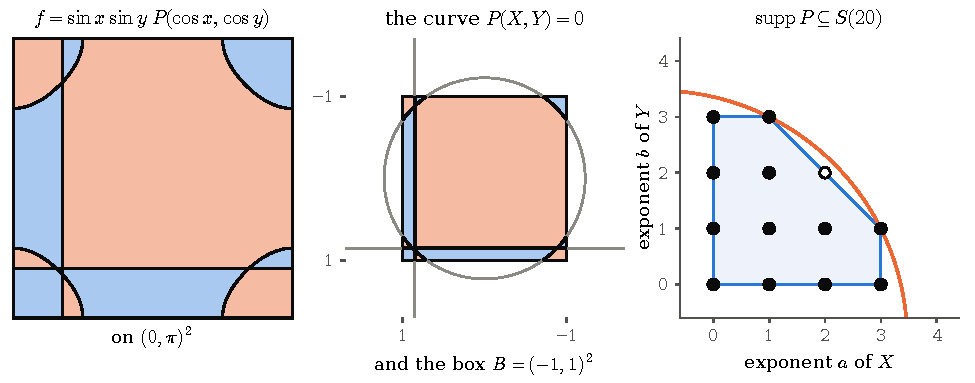
\includegraphics[width=0.96\textwidth]{fig_reduction.pdf}
\caption{The reduction for
$P=(X-\tfrac{17}{20})(Y-\tfrac{17}{20})(X^2+Y^2-\tfrac32)$, a maximiser at $\lambda=20$.
Left: the combination $f$ on $(0,\pi)^2$. Middle: the real curve $P=0$. The nodal set of $f$
is the part of this curve inside the box $B$ (the axes are reversed because the cosine is
decreasing). Right: the exponents of $P$ (filled) among the points of $S(20)$, which are the
lattice points $(a,b)$ with $(a+1)^2+(b+1)^2\le20$. The polygon is $\Delta_{20}$.}
\label{fig:reduction}
\end{figure}

\subsection{Lattice polygons}
A \emph{down-closed lattice polygon} is a convex lattice polygon $D\subseteq\R_{\ge0}^2$
(possibly a point or a segment) with $\down D=D$, where
$\down A=(A-\R^2_{\ge0})\cap\R^2_{\ge0}$. For such $D$ we write $I(D)$ for the number of
interior lattice points (zero for points and segments), $w_x(D)=\max_Dx$ and
$w_y(D)=\max_Dy$ for its widths, and $w(D)=w_x(D)+w_y(D)$. The mixed area is
$\MV(A,B)=\operatorname{area}(A+B)-\operatorname{area}(A)-\operatorname{area}(B)$,
normalised so that two unit segments in different directions have $\MV=1$.

\subsection{The corner-sign number}
\begin{definition}\label{def:cap}
Let $A\subset\Z_{\ge0}^2$ be finite, $d_x=\max\{a:(a,b)\in A\}$ and
$d_y=\max\{b:(a,b)\in A\}$. The \emph{top row} of $A$ is \emph{even} if $a$ is even for every
$(a,d_y)\in A$, and the \emph{right column} is \emph{even} if $b$ is even for every
$(d_x,b)\in A$. For $d\ge0$ and signs $u,v,s\in\{\pm1\}$ put
$\beta(d;u,v;s)=d-[v\ne s]-[u\ne(-1)^ds]$ if $d\ge1$ and $\beta=0$ if $d=0$. Then
$\capn(A)$ is the maximum, over corner signs $\sigma\in\{\pm1\}^{\{\pm1\}^2}$ and side signs
$R,L,T,B'\in\{\pm1\}$, of
\[
\beta(d_y;\sigma_{1,-1},\sigma_{1,1};R)+\beta(d_y;\sigma_{-1,-1},\sigma_{-1,1};L)
+\beta(d_x;\sigma_{-1,1},\sigma_{1,1};T)+\beta(d_x;\sigma_{-1,-1},\sigma_{1,-1};B'),
\]
subject to $L=R$ if the top row is even, and $B'=T$ if the right column is even.
\end{definition}

The four terms correspond to the sides $X=1$, $X=-1$, $Y=1$, $Y=-1$ of $B$. Here $\sigma$ records
the signs of a polynomial at the corners, and $R,L,T,B'$ the signs of the leading
coefficients of its restrictions to the sides (Lemma~\ref{lem:cap}).

\subsection{The bound}
\begin{definition}\label{def:U}
Let $\mathcal D_\lambda$ be the set of down-closed lattice polygons $D\subseteq\Delta_\lambda$
that are neither a point nor an axis segment of lattice length at least~$2$. For
$D\in\mathcal D_\lambda$ let
\[
h(D)=\begin{cases}1, & D=\conv\{0,e_1,e_2\},\\
n, & D=\conv\{0,e_1,ne_2\}\text{ or }\conv\{0,ne_1,e_2\},\ n\ge2,\\
w(D), & \text{otherwise,}\end{cases}
\]
and $\eta(D)=\min\bigl(h(D),\lfloor\capn(D\cap\Z^2)/2\rfloor\bigr)$.
For a multiset $D_1,\dots,D_k\in\mathcal D_\lambda$ with $D_1+\dots+D_k\subseteq\Delta_\lambda$,
put $c_\lambda=\lfloor\capn(S(\lambda))/2\rfloor$ and
\begin{equation}\label{eq:Umulti}
U(D_1,\dots,D_k)=1+\sum_{i}\bigl(I(D_i)+1\bigr)+\sum_{i<j}\MV(D_i,D_j)
+\max_{T\subseteq\{1,\dots,k\}}\Bigl(\min\Bigl(c_\lambda,\sum_{i\in T}\eta(D_i)\Bigr)-|T|\Bigr).
\end{equation}
Finally, $U(\lambda)$ is the maximum of $U(D_1,\dots,D_k)$ over all such multisets. The empty
multiset gives $U=1$.
\end{definition}

The multiset is finite because each $D\in\mathcal D_\lambda$ contains $0$ and has positive
width, so at most $w(\Delta_\lambda)$ polygons fit. Thus $U(\lambda)$ is a well-defined
integer.

\begin{theorem}[Theorem A]\label{thm:main}
For every $\lambda>0$ and every $0\ne f\in E_\lambda$, $\nu(f)\le U(\lambda)$.
\end{theorem}

The proof will take up the next three sections. By \eqref{eq:reduction}, it is enough to show $\nu_B(P)\le U(\lambda)$ for every $0\ne P$ with $\supp P\subseteq S(\lambda)$.

%=====================================================================================
\section{Normalisations}\label{sec:normal}

In this section we put $P$ into a normal form that will make the counting arguments of
Section~\ref{sec:inputs} easier. We shrink the box slightly so that the nodal set behaves well
at the boundary, and we replace the factors of $P$ by simple lattice polygons.

\begin{lemma}[Generic box]\label{lem:box}
Let $0\ne P$ have support in $S(\lambda)$. There are $r_x,r_y\in(0,1)$ such that
$P'(X,Y)=P(r_xX,r_yY)$ satisfies:
\begin{enumerate}[label=(\alph*),nosep]
\item $\supp P'=\supp P$;
\item $\nu_B(P)\le\nu_B(P')$;
\item no corner of $\bar B$ lies on $Z(P')$, no side line of $B$ is contained in $Z(P')$,
and $Z(P')$ is not tangent to any side of $B$.
\end{enumerate}
\end{lemma}

\begin{proof}
A diagonal scaling multiplies each coefficient $c_{a,b}$ by $r_x^ar_y^b\ne0$, which gives (a).
(A translation would not do: it can create monomials of the wrong parity, which matters
for Lemma~\ref{lem:cap}.)

The set $B\setminus Z(P)$ is semialgebraic, so it has finitely many components, so we can choose one
point in each. For $(r_x,r_y)$ close enough to $(1,1)$, the box
$R=(-r_x,r_x)\times(-r_y,r_y)$ contains all of these points. Points in different
components of $B\setminus Z(P)$ lie in different components of the smaller set
$R\setminus Z(P)$, so $\nu_B(P)\le\#\pi_0(R\setminus Z(P))=\nu_B(P')$, which is (b).

For each choice of signs, $P(\pm r_x,\pm r_y)=0$ defines a proper algebraic subset of the
$(r_x,r_y)$-plane, since $P\ne0$. A line $\{X=c\}$ lies in $Z(P)$ for only finitely many
$c$, and $Z(P)$ is tangent to vertical lines only at finitely many $X$-values (the critical
values of $X$ on the components of $Z(P)$ that are not vertical lines). The same holds for
horizontal lines. So a generic choice of $(r_x,r_y)$ near $(1,1)$ also gives (c).
\end{proof}

From now on $P$ is in this normal form. Only the support of $P$ enters the corner-sign
argument, and on the shrunk box the leading coefficient of $P(\pm r_x,Y)$ in $Y$ is
$\sum_ac_{a,d_y}(\pm r_x)^a$, which is the same for both signs when the top row is even.
So nothing changes when the corners are moved from $(\pm1,\pm1)$ to $(\pm r_x,\pm r_y)$, and we
keep writing $B$ for the box.

\subsection{Factors}
Write $P=c\prod_iF_i^{m_i}$ with the $F_i$ irreducible over $\R$ and pairwise non-associate.
Then $Z(P)=\bigcup_iZ(F_i)$, so the multiplicities $m_i$ do not affect the nodal set. We
discard two kinds of factors without changing $\nu_B(P)$:
\begin{itemize}[nosep]
\item factors that are irreducible over $\R$ but not over $\C$: then $F_i=G\bar G$ with
$G,\bar G$ non-associate, so $Z(F_i)\subseteq Z(G)\cap Z(\bar G)$ is finite, and removing
finitely many points from a planar open set does not change the number of its components;
\item factors without zeros in $\bar B$.
\end{itemize}
The remaining factors are irreducible over $\C$ and have real zeros in $\bar B$. A
univariate polynomial that is irreducible over $\C$ is linear, so each remaining factor is
either a line $X-a$ or $Y-b$, or genuinely bivariate. Write $N(F)$ for the Newton polygon
of $F$.

\begin{lemma}[Down-closures]\label{lem:down}
Put $D_i=\down N(F_i)$. Then:
\begin{enumerate}[label=(\alph*),nosep]
\item each $D_i$ is a down-closed lattice polygon containing $0$, and $D_i\in\mathcal D_\lambda$;
\item $D_1+\dots+D_k\subseteq\Delta_\lambda$;
\item the side degrees of $F_i$ (the degrees of $F_i(\pm1,Y)$ in $Y$ and of
$F_i(X,\pm1)$ in $X$) are at most $w_y(D_i)$ and $w_x(D_i)$, and
$\capn(\supp F_i)\le\capn(D_i\cap\Z^2)$.
\end{enumerate}
\end{lemma}

\begin{proof}
(a) For a convex lattice polygon $A$ in the quadrant, $\down A$ is the convex hull of $A$,
of the projections of its vertices to both axes, and of $0$. So it is a down-closed lattice
polygon containing $0$. It is a point only if $F_i$ is constant, and an axis segment of
length at least $2$ only if $F_i$ is univariate of degree at least~$2$. Both cases were excluded.
Membership in $\mathcal D_\lambda$ then follows from (b).

(b) If $u\le a$ and $u'\le a'$ coordinatewise then $u+u'\le a+a'$, so
$\down A+\down A'\subseteq\down(A+A')$. Since $0\in D_i$, adding summands only enlarges a
Minkowski sum. Let $G$ be the product of the discarded factors, with their multiplicities, so
that $N(P)=N(G)+\sum_im_iN(F_i)$. Since $N(G)$ lies in the quadrant, adding it only enlarges
the down-closure. Hence
\[
\sum_iD_i\subseteq\sum_im_iD_i\subseteq\down\Bigl(\sum_im_iN(F_i)\Bigr)\subseteq\down N(P)
\subseteq\Delta_\lambda,
\]
because $N(P)\subseteq\Delta_\lambda$ and $\Delta_\lambda$ is down-closed.

(c) Down-closure does not change the maximal coordinates. The number $\capn(A)$ depends only on
$(d_x,d_y)$, which are the same for $\supp F_i$ and $D_i\cap\Z^2$, and on the two parity
constraints. The top row of $D_i\cap\Z^2$ contains that of $\supp F_i$, so if the former is
even so is the latter, and the same is true for the right column. Hence the constraints for $D_i$ are
weaker, and the maximum can only grow.
\end{proof}

\subsection{Torus coordinates}
Put $\tilde F(X,Y)=F(X-3,Y-3)$. Then $\bar B$ corresponds to $[2,4]^2$, which lies in the
positive real torus $(\R_{>0})^2\subset(\C^*)^2$. Expanding $(X-3)^a(Y-3)^b$ produces only
monomials below $(a,b)$, so $N(\tilde F)\subseteq\down N(F)$. This shift is used only to make
every point of $\bar B$ a torus point. The parity arguments are applied to the unshifted
polynomials.

%=====================================================================================
\section{The topological count and the local inputs}\label{sec:inputs}

We now collect the tools for the proof of Theorem~A. We start with an exact formula for the
number of nodal domains, and then bound each of its terms in turn.

\subsection{An Euler formula}
For $p\in B$ let $h_p$ be the number of half-branches of $Z=Z(P)$ at $p$. By the local conic
structure of semialgebraic sets, $Z$ is a cone over $h_p$ points near $p$. For
$q\in Z\cap\partial B$ let $e_q$ be the number of half-branches of $Z$ at $q$ that lie in
$B$, and put $\varepsilon=\sum_qe_q$ (the number of \emph{ends}). Let $C$ be the number of
connected components of $Z$ that are contained in $B$ and are not points.

\begin{lemma}[Euler formula]\label{lem:euler}
Let $P\ne0$ be a polynomial such that no side of $B$ is contained in $Z(P)$. Then
$\displaystyle\nu_B(P)=1+\frac{\varepsilon}{2}+\sum_{p\in\Sigma}\Bigl(\frac{h_p}{2}-1\Bigr)+C$,
where $\Sigma$ is the set of points $p\in Z\cap B$ with $h_p\notin\{0,2\}$.
\end{lemma}

\begin{proof}
Let $K=(Z\cap\bar B)\cup\partial B$, a compact semialgebraic subset of $\R^2\subset S^2$. By
Alexander duality, $S^2\setminus K$ has $1+b_1(K)$ components. One of them is the exterior of
$\bar B$, and the others are the components of $B\setminus Z$. So $\nu_B(P)=b_1(K)$.

The set $K$ is a finite graph. Take as vertices the points of $\Sigma$, the isolated points of
$Z\cap B$, the points of $Z\cap\partial B$, the four corners, and one extra point on each
component of $Z\cap B$ that is a circle without other vertices. The degrees are $h_p$ for
$p\in\Sigma$, $0$ for isolated points, $e_q+2$ for $q\in Z\cap\partial B$ (two edges run
along $\partial B$, and no half-branch runs along $\partial B$ because no side lies in $Z$;
this includes a corner that lies on $Z$), and $2$ for the other corners and the extra points. By the handshake lemma,
\[
\#\text{edges}-\#\text{vertices}=\sum_{p\in\Sigma}\Bigl(\frac{h_p}{2}-1\Bigr)+\frac{\varepsilon}{2}
-\#\{\text{isolated points}\}.
\]
A component of $Z\cap\bar B$ that misses $\partial B$ is open and closed in $Z$, so the
number of components of $K$ is $1+C+\#\{\text{isolated points}\}$. Since
$b_1=\#\text{edges}-\#\text{vertices}+\#\text{components}$, the formula follows.
\end{proof}

\begin{figure}[t]
\centering
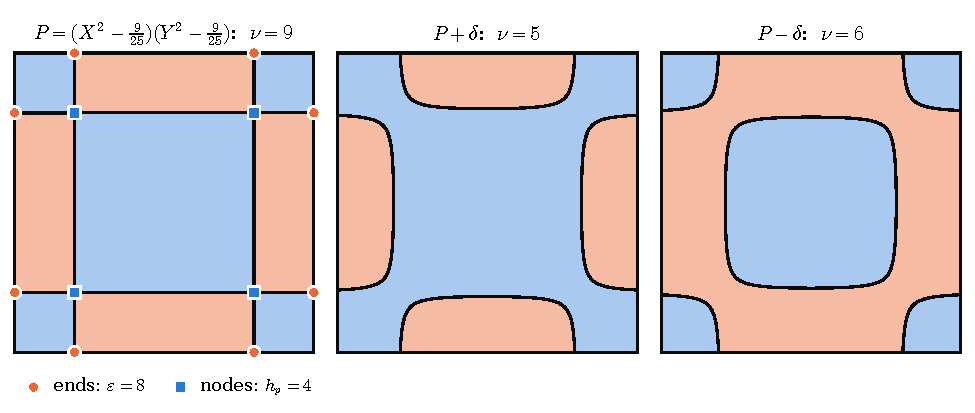
\includegraphics[width=0.96\textwidth]{fig_euler.pdf}
\caption{The Euler formula at $\lambda=18$. Left: the curve of
$P=(X^2-\tfrac9{25})(Y^2-\tfrac9{25})$ has $\varepsilon=8$ ends and four nodes with $h_p=4$,
so $\nu=1+\tfrac82+4=9$. Middle and right: for $\delta=0.012$ the curves of $P\pm\delta$ are
smooth, the nodes are gone, and only $5$ or $6$ domains are left. The maximisers are
degenerate curves (Remark~\ref{rem:degenerate}).}
\label{fig:euler}
\end{figure}

\subsection{Ends}
\begin{lemma}[Ends and side roots]\label{lem:ends}
Let $F$ be a polynomial, $q\in Z(F)\cap\partial B$ not a corner, and $\ell$ the side line
through $q$, with $\ell\not\subseteq Z(F)$. Then the number of half-branches of $Z(F)$ at
$q$ that lie in $B$ is at most $\operatorname{ord}_q(F|_\ell)$. Consequently, if no corner
of $\bar B$ lies on $Z(F)$ and no side line is contained in $Z(F)$, the number
$\varepsilon_F$ of ends of $Z(F)$ is at most the number of roots, counted with multiplicity,
of the four side restrictions of $F$ in the open sides.
\end{lemma}

\begin{proof}
We use two standard facts about the local branches of a real plane curve at $q$
\cite[\S3]{Milnor}: (i) a complex branch $\beta$ with $\bar\beta\ne\beta$ has no real points
near $q$ other than $q$, since its real points lie in $\beta\cap\bar\beta=\{q\}$; (ii) a
conjugation-invariant branch has a primitive Puiseux parametrisation $\gamma$ with real
coefficients, and its real locus near $q$ is exactly $\gamma((-\delta,\delta))$. (If
$\bar\gamma(t)=\gamma(\zeta t)$ with $\zeta^n=1$, the substitution $t=\omega s$ with
$\omega^2=\zeta$ makes the coefficients real, and primitivity excludes real points coming
from non-real $s$.)

Let $L$ be an affine function with $\ell=\{L=0\}$ and $L>0$ on $B$. By (i) and (ii), every
real half-branch at $q$ is $\gamma|_{(0,\delta)}$ or $\gamma|_{(-\delta,0)}$ for a real
branch $\gamma$, and
$\operatorname{ord}_q(F|_\ell)=I_q(Z(F),\ell)=\sum\operatorname{ord}_tL(\gamma(t))$, the sum
running over all complex branches. A half-branch lies in $B$ exactly when $L\circ\gamma>0$ on
it. If both halves of a real branch lie in $B$, then $L\circ\gamma$ has even order, hence
order at least $2$. So each real branch contributes at most $\operatorname{ord}_tL\circ\gamma$
half-branches in $B$, and non-real branches contribute none. If $F$ is not reduced, a factor
of multiplicity $m$ multiplies its contribution to $\operatorname{ord}_q(F|_\ell)$ by $m$
without changing $Z(F)$, so the inequality persists.
\end{proof}

\subsection{Corner signs}
\begin{lemma}[Roots and corner signs]\label{lem:roots}
Let $g\in\R[t]$ with $\deg g\le d$ and $g(\pm1)\ne0$, let $g_d$ be the coefficient of $t^d$,
and let $s$ be the sign of $g_d$ when $g_d\ne0$. Then the number of roots of $g$ in $(-1,1)$,
counted with multiplicity, is at most
\[
d-[\operatorname{sgn}g(1)\ne s]-[\operatorname{sgn}g(-1)\ne(-1)^ds].
\]
If $g_d=0$, it is at most $d-1$.
\end{lemma}

\begin{proof}
If the signs of $g$ at $1$ and at $+\infty$ differ, then $g$ has a root in $(1,\infty)$.
Likewise on $(-\infty,-1)$, where the sign at $-\infty$ is $(-1)^ds$. The total number of
roots is at most $d$.
\end{proof}

This lemma is formalised in Lean~4 with Mathlib (Appendix~\ref{app:code}).

\begin{lemma}[Corner cap]\label{lem:cap}
If $\supp F\subseteq A$ and no corner of $\bar B$ lies on $Z(F)$, then
$\varepsilon_F\le\capn(A)$.
\end{lemma}

\begin{proof}
The restriction $F(\pm1,Y)$ has degree at most $d_y$, and its $Y^{d_y}$-coefficient is
$\sum_a(\pm1)^ac_{a,d_y}$, and these two coefficients are equal when the top row is even.
Likewise for $F(X,\pm1)$ and the right column. Apply Lemma~\ref{lem:ends} and then
Lemma~\ref{lem:roots} on each side. If a leading coefficient vanishes, the maximum in
Definition~\ref{def:cap} still dominates. If the coefficient on one side vanishes and is not
shared, that side contributes at most $d-1$ roots, and for the given corner signs the two
choices of its sign have mismatch counts adding up to $2$, so one of them gives at least
$d-1$. If the shared coefficient on $X=\pm1$ vanishes, these two sides contribute at most
$2d_y-2$, and the two choices of the shared sign $R=L$ have mismatch counts adding up to $4$,
so one of them gives at least $2d_y-2$. The sides $Y=\pm1$ are treated in the same way.
\end{proof}

Figure~\ref{fig:corner} illustrates the two lemmas for cubic restrictions, which is the case
of $S(17)$ and $S(18)$.

\begin{figure}[t]
\centering
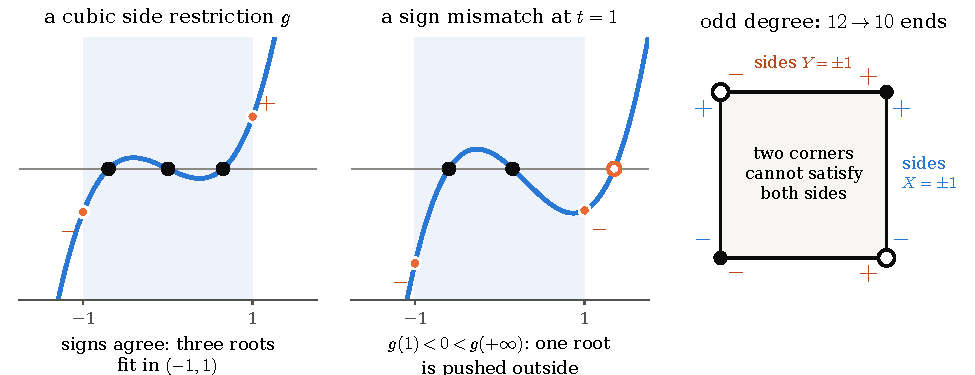
\includegraphics[width=0.96\textwidth]{fig_corner.pdf}
\caption{The corner-sign argument. Left and middle: a cubic $g$ with positive leading
coefficient can have three roots in $(-1,1)$ only if $g(1)>0$ and $g(-1)<0$; each mismatch
pushes a root outside (Lemma~\ref{lem:roots}). Right: when the top row and the right column
are even and both side degrees are odd, the sides $X=\pm1$ ask for one sign pattern at the
corners (blue signs) and the sides $Y=\pm1$ for another (orange signs), drawn here for
positive leading coefficients. They disagree at two corners (open circles) whatever the
leading signs are, so cubic sides carry at most $10$ ends instead of $12$.}
\label{fig:corner}
\end{figure}

\begin{lemma}[Graph-type factors]\label{lem:graph}
If $\down N(F)=\conv\{0,e_1,ne_2\}$ then $\varepsilon_F\le2n$; if $\down N(F)$ is the unit
triangle then $\varepsilon_F\le2$. The same holds with the coordinates exchanged.
\end{lemma}

\begin{proof}
In the first case $F=\alpha X+q(Y)$ with $\deg q\le n$ and $\alpha\ne0$, so $Z(F)$ is the graph
$X=\varphi(Y)$ of $\varphi=-q/\alpha$. Its arcs in $B$ correspond to the components of
$J=\{Y\in(-1,1):|\varphi(Y)|<1\}$, with two ends each. The function $\varphi$ has at most $n$
monotone pieces on $(-1,1)$, each meeting $J$ in at most one interval, so $J$ has at most $n$
components. In the second case $Z(F)$ is a line, which meets the convex curve $\partial B$
at most twice.
\end{proof}

\subsection{Harnack and genus}
\begin{lemma}\label{lem:harnack}
Let $F$ be one of the remaining factors, with $D=\down N(F)$. For $p\in B$ let $r_p$ be the
number of real branches of $Z(F)$ at $p$, and let $C_F$ be the number of components of $Z(F)$
contained in $B$ that are not points. Then
\[
C_F+\sum_{p\in B}(r_p-1)^+\le I(D)+1-[\varepsilon_F>0].
\]
\end{lemma}

\begin{proof}
We work with $\tilde F$, which is irreducible over $\C$, and with $N=N(\tilde F)\subseteq D$.
Every point of $\bar B$ is a point of the torus in these coordinates. The polygon $N$ is not
a point, because then $\tilde F$ would be a monomial and $F$ would have no zeros in $\bar B$.

If $N$ is a segment with primitive direction $(p,\pm q)$, then $\tilde F$ is a monomial times
a univariate polynomial in $t=X^pY^{\pm q}$, which is linear by irreducibility over $\C$. So
$Z(\tilde F)\cap(\C^*)^2$ is a smooth rational curve, and $r_p\le1$. Its real points in the
positive quadrant form at most one unbounded arc, so $C_F=0$. Thus the left side is $0$, and
the inequality holds. (A binomial curve in the original coordinates, such as $X^p=cY^q$, is not a
binomial after the shift, so it falls under the general case.)

Otherwise let $X_N$ be the projective toric surface of $N$ and $L_N$ its ample line bundle,
whose sections are spanned by the monomials with exponents in $N$. Since $N(\tilde F)=N$, the
section $\tilde F$ does not vanish identically on any boundary divisor, so its divisor is the
closure $\bar{\mathcal C}$ of the torus curve, an integral Cartier divisor. Its arithmetic
genus depends only on the class of $L_N$, and a generic member of $|L_N|$ is smooth of genus
$I(N)$ \cite{Khovanskii}. Hence $p_a(\bar{\mathcal C})=I(N)$. If $g$ denotes the geometric
genus, then $p_a=g+\sum_p\delta_p$, so
\[
g+\sum_{p\in(\C^*)^2}\delta_p\le I(N)\le I(D)
\]
(see also \cite{Beelen} for the bound $g\le I(N)$). Every $p\in B$ is a torus
point, and $\delta_p\ge r_p-1$.

By Harnack's theorem \cite{Harnack} the real part of the normalisation has at most $g+1$
components. Each non-point component of $Z(F)$ in $B$ is the image of a nonempty union of
components of the real normalisation, distinct components using disjoint unions; and if
$\varepsilon_F>0$, a further component maps onto a branch reaching $\partial B$. Hence
$C_F\le g+1-[\varepsilon_F>0]$. Adding $\sum_{p\in B}(r_p-1)^+\le\sum_p\delta_p\le I(D)-g$
gives the claim.
\end{proof}

\begin{example}
The shift matters. The polynomial $F=X^3+X^2-Y^2$ (supported in $S(17)$) has a real node at
the origin. Its own Newton polygon $\conv\{(3,0),(2,0),(0,2)\}$ has no interior lattice point,
and on its toric surface the origin lies on a boundary divisor. After the shift,
$N(\tilde F)=\conv\{0,(3,0),(0,2)\}$ has one interior point and the node is a torus point.
\end{example}

\begin{lemma}[Bernstein]\label{lem:bernstein}
For $i\ne j$, $\#\bigl(Z(F_i)\cap Z(F_j)\cap B\bigr)\le\MV(D_i,D_j)$.
\end{lemma}

\begin{proof}
The factors have no common component, so these are isolated common zeros of
$\tilde F_i,\tilde F_j$ in $(\C^*)^2$. Apply the Bernstein--Kushnirenko theorem
\cite{Bernstein,Kushnirenko} and the monotonicity of $\MV$ under inclusion.
\end{proof}

%=====================================================================================
\section{Proof of Theorem A}\label{sec:proofA}

We can now put the pieces together.
Let $F_1,\dots,F_k$ be the remaining factors and $D_i=\down N(F_i)$. At $p\in\Sigma$ let
$r_{i,p}$ be the number of real branches of $Z(F_i)$ at $p$ and $m_p$ the number of $i$ with
$r_{i,p}\ge1$. Each real branch contributes two half-branches, so
\[
\frac{h_p}{2}-1=\sum_ir_{i,p}-1=\sum_i(r_{i,p}-1)^++(m_p-1),\qquad
m_p-1\le\#\{i<j:p\in Z(F_i)\cap Z(F_j)\}.
\]
Every non-point component of $Z$ in $B$ contains a non-point component of some $Z(F_i)$ in
$B$, and different components of $Z$ contain different ones, so $C\le\sum_iC_{F_i}$. Distinct
factors share no half-branch, so $\varepsilon=\sum_i\varepsilon_{F_i}$. Lemma~\ref{lem:euler}
together with Lemmas~\ref{lem:harnack} and~\ref{lem:bernstein} gives
\begin{equation}\label{eq:mainineq}
\nu_B(P)\le1+\sum_i\Bigl(\frac{\varepsilon_{F_i}}{2}+I(D_i)+1-[\varepsilon_{F_i}>0]\Bigr)
+\sum_{i<j}\MV(D_i,D_j).
\end{equation}
Each $\varepsilon_{F_i}$ is even (apply Lemma~\ref{lem:euler} to $F_i$ alone, and recall that
every $h_p$ is even). By
Lemmas~\ref{lem:ends}, \ref{lem:cap}, \ref{lem:graph} and~\ref{lem:down}(c),
$\varepsilon_{F_i}/2\le\eta(D_i)$: the side degrees are at most the widths of $D_i$, the
graph-type cases are covered by Lemma~\ref{lem:graph}, and the corner cap of $\supp F_i$ is at
most that of $D_i\cap\Z^2$. (The zero set of $F_i$ misses the corners because it is contained
in $Z(P)$.) Applying Lemma~\ref{lem:cap} to $P$ itself, with $A=S(\lambda)$, gives
$\sum_i\varepsilon_{F_i}=\varepsilon\le\capn(S(\lambda))$, hence
$\varepsilon/2\le c_\lambda$ since $\varepsilon$ is even. With $T=\{i:\varepsilon_{F_i}>0\}$,
\[
\sum_i\Bigl(\frac{\varepsilon_{F_i}}{2}-[\varepsilon_{F_i}>0]\Bigr)
\le\min\Bigl(c_\lambda,\sum_{i\in T}\eta(D_i)\Bigr)-|T|,
\]
so the right side of \eqref{eq:mainineq} is at most $U(D_1,\dots,D_k)$. By
Lemma~\ref{lem:down}(a),(b) this multiset is admissible, so it is at most $U(\lambda)$.
\qed

\begin{remark}[Degenerate curves]\label{rem:degenerate}
None of the arguments above assume that $Z(P)$ is smooth, irreducible or in general position.
This is important, because the maximisers tend to be degenerate. For example, at $\lambda=18$, $(X^2-\tfrac{9}{25})(Y^2-\tfrac{9}{25})$ has
$9$ nodal domains, while small generic perturbations have $5$ or $6$. Multiple factors are
handled by passing to the radical; singular points of one factor are paid for by $\delta_p$
in Lemma~\ref{lem:harnack}; crossings of several factors, including tangential ones, by
Bernstein's theorem (which counts with multiplicity); and contacts with the boundary are made
transversal and corner-free by Lemma~\ref{lem:box}. For the example above, $\varepsilon=8$,
there are four nodes with $h_p=4$, and $\nu=1+4+4=9$. In fact, every inequality in the proof is an
equality.
\end{remark}

%=====================================================================================
\section{An identity for the bound, and the Courant--Herrmann bound}\label{sec:identity}

In this section we show that $U(\lambda)$ is never larger than $\dim E_\lambda$. The key step is
an exact identity, which writes $U$ in terms of lattice points and lattice perimeters. We first
need some notation.

For a lattice polygon or lattice segment $A$ let $B^*(A)$ be its lattice perimeter (the
number of primitive lattice segments on its boundary, where a segment of lattice length $\ell$ has
$B^*=2\ell$), and let $I^*(A)=\operatorname{area}(A)-B^*(A)/2+1$. By Pick's theorem
$I^*(A)=I(A)$ for two-dimensional $A$, $I^*=0$ for a unit segment, and
$\#(A\cap\Z^2)=I^*(A)+B^*(A)$ in all cases.

The \emph{upper chain} of a down-closed lattice polygon $D$ is its boundary minus the two
axis edges. Its lattice length is $B^*(D)-w(D)$ (for a unit segment, the convention
$B^*=2$ gives upper chain length $1$).

\begin{proposition}\label{prop:identity}
For every admissible multiset with $D=D_1+\dots+D_k$, writing $w_i=w(D_i)$ and $G$ for the
maximum over $T$ in \eqref{eq:Umulti},
\begin{equation}\label{eq:identity}
U(D_1,\dots,D_k)=\#(D\cap\Z^2)-\sum_i\bigl(B^*(D_i)-w_i-1\bigr)-\Bigl(\sum_i(w_i-1)-G\Bigr),
\end{equation}
and all three subtracted quantities are non-negative. In particular $U(\lambda)\le N(\lambda)$.
\end{proposition}

\begin{proof}
Lattice perimeter is additive under Minkowski sums, because the edge vectors are
concatenated, and $\operatorname{area}(A+A')=\operatorname{area}A+\operatorname{area}A'+\MV(A,A')$.
Hence $I^*(A+A')=I^*(A)+I^*(A')+\MV(A,A')-1$, and by induction
\[
1+\sum_i\bigl(I(D_i)+1\bigr)+\sum_{i<j}\MV(D_i,D_j)=I^*(D)+2k
=\#(D\cap\Z^2)-\sum_i\bigl(B^*(D_i)-2\bigr),
\]
which is \eqref{eq:identity}. The upper chain of $D_i$ has length at least $1$, so
$B^*(D_i)\ge w_i+1$. Next, $\eta(D_i)\le h(D_i)\le w_i$, hence
$G\le\max_T\sum_{i\in T}(\eta(D_i)-1)\le\sum_i(w_i-1)$, using $w_i\ge1$. Finally
$D\subseteq\Delta_\lambda$ and $\Delta_\lambda\cap\Z^2=S(\lambda)$, so
$\#(D\cap\Z^2)\le N(\lambda)$.
\end{proof}

\begin{theorem}[Theorem B]\label{thm:CH}
For every $\lambda$, every $0\ne f\in E_\lambda$ has at most $\dim E_\lambda$ nodal domains.
Consequently, whenever $\lambda_n<\lambda_{n+1}$, every nonzero combination of
$u_1,\dots,u_n$ has at most $n$ nodal domains.
\end{theorem}

\begin{proof}
Combine Theorem~\ref{thm:main} with Proposition~\ref{prop:identity}. If
$\lambda_n<\lambda_{n+1}$ then $\operatorname{span}(u_1,\dots,u_n)=E_{\lambda_n}$ has dimension $n$.
\end{proof}

The extended Courant property at $\lambda$ requires the stronger inequality
$U(\lambda)\le\kappa(\lambda)=N(\lambda)-(r(\lambda)-1)$. By \eqref{eq:identity}, the
\emph{deficiency} $N(\lambda)-U(D_1,\dots,D_k)$ of an admissible multiset is the sum of
\begin{enumerate}[nosep]
\item $\miss(D):=\#(S(\lambda)\setminus D)$, the lattice points of $S(\lambda)$ not reached;
\item the excess lengths $B^*(D_i)-w_i-1$ of the upper chains;
\item the loss $\sum_i(w_i-1)-G$ in the ends term, which comes from graph-type factors and
from the corner caps.
\end{enumerate}
Notice that every point $(m-1,k-1)$ with $m^2+k^2=\lambda$ lies on the boundary arc of
$S(\lambda)$. In other words, ECP at $\lambda$ asks that these three terms together make up for
the $r(\lambda)$ new lattice points on the arc. Figure~\ref{fig:polygons} shows the three
terms for the maximisers at $\lambda=17$ and $18$.

\begin{figure}[t]
\centering
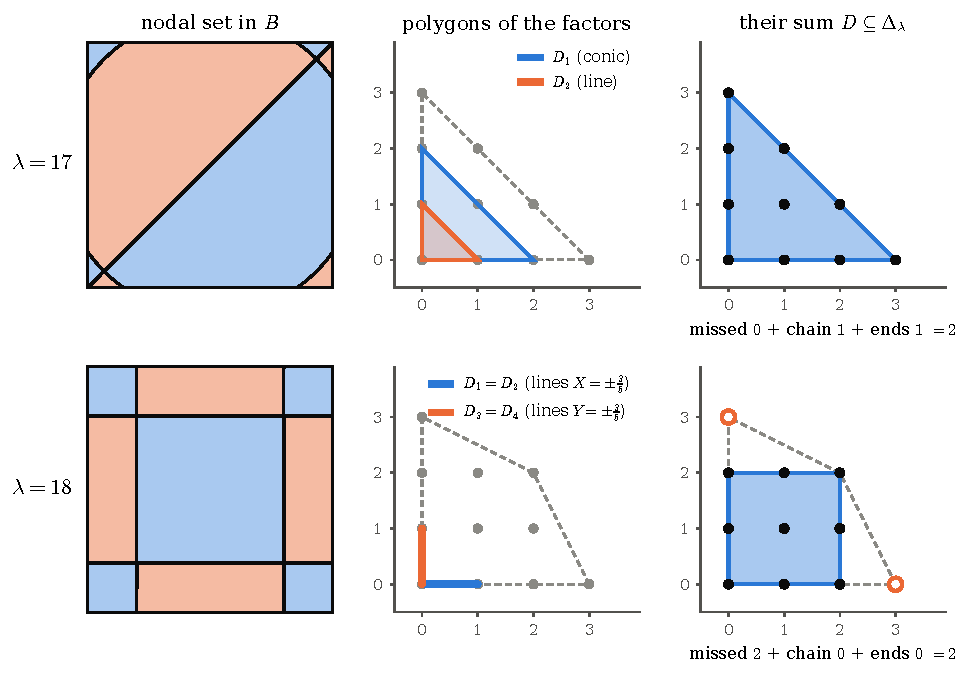
\includegraphics[width=0.9\textwidth]{fig_polygons.pdf}
\caption{From the curve to lattice polygons, for the maximisers of
Proposition~\ref{prop:17-18}. Left: the nodal set. Middle: the polygons $D_i$ of the factors
inside $\Delta_\lambda$ (dashed). Right: their Minkowski sum $D$; open circles are the points
of $S(\lambda)$ that $D$ misses. Below each row is the deficiency $N(\lambda)-U(D_1,\dots,D_k)$,
split into the three terms above. At $\lambda=17$ the sum fills $\Delta_{17}$, but the conic
has an upper chain of length $2$ and the ends term loses $1$. At $\lambda=18$ nothing is lost
except the two missed points.}
\label{fig:polygons}
\end{figure}

%=====================================================================================
\section{A lower bound for the deficiency}\label{sec:deficiency}

We now turn to ECP itself. By the discussion at the end of the last section, we need to show
that the gap $N(\lambda)-U(\lambda)$ is at least $r(\lambda)-1$. The main goal of this section is
to bound this gap from below by a quantity that only depends on the shape of $S(\lambda)$.

A primitive lattice segment of the upper chain of a down-closed polygon is \emph{slanted} if
its direction is $(-a,b)$ with $a,b\ge1$, and \emph{axis-parallel} otherwise. The
\emph{class} of a slanted primitive segment is $(a\bmod2,b\bmod2)\in(\Z/2)^2$, which is nonzero
since $\gcd(a,b)=1$. For a down-closed polygon $D$ let $n(D)$ be the number of slanted
primitive segments of its upper chain and $\sigma(D)\in(\Z/2)^2$ the sum of their classes.

\begin{lemma}[Parity cap loss]\label{lem:paritycap}
Let $D\in\mathcal D_\lambda$ be two-dimensional, with every primitive segment of its upper
chain slanted, and with $(w_x,w_y)\not\equiv(0,0)\pmod2$. Then $\capn(D\cap\Z^2)\le2w(D)-1$,
so $\eta(D)\le w(D)-1$.
\end{lemma}

\begin{proof}
The chain begins and ends with slanted segments, so the top row of $D\cap\Z^2$ is
$\{(0,w_y)\}$ and the right column is $\{(w_x,0)\}$. Both are even, so both constraints of
Definition~\ref{def:cap} apply: $L=R$ and $B'=T$. Suppose that all eight mismatch indicators
vanish. If $w_y$ is odd, the side $X=1$ gives $\sigma_{1,1}=R=-\sigma_{1,-1}$, while the sides
$Y=\pm1$ give $\sigma_{1,1}=T=\sigma_{1,-1}$, a contradiction. If $w_y$ is even, all four
corner signs equal $R$, and the side $Y=1$ forces $(-1)^{w_x}=1$, so $w_x$ is even, contrary to
the hypothesis. Hence some indicator equals $1$ and $\capn\le2w-1$.
\end{proof}

\begin{lemma}[Cost of a factor]\label{lem:factorcost}
For $D_i\in\mathcal D_\lambda$ put
$c_i=\bigl(B^*(D_i)-w_i-1\bigr)+\bigl(w_i-\max(\eta(D_i),1)\bigr)$; both brackets are
non-negative. If $n_i=n(D_i)\ge1$, then $c_i\ge n_i-1+[\sigma(D_i)\ne0]$.
\end{lemma}

\begin{proof}
The first bracket is the lattice length of the upper chain minus $1$. If the chain contains
an axis-parallel segment, it has at least $n_i+1$ segments, so the first bracket is at least
$n_i$. Otherwise the first bracket equals $n_i-1$, and we must show that the second bracket is
positive when $\sigma(D_i)\ne0$. In that case $(w_x,w_y)=\sum(a,b)\not\equiv(0,0)$. If $D_i$ is
of graph type or the unit triangle, then $h(D_i)=w_i-1$. Otherwise
Lemma~\ref{lem:paritycap} applies. Either way $\eta(D_i)\le w_i-1$.
\end{proof}

\begin{lemma}[Grouping]\label{lem:grouping}
Partition a multiset of $T$ slanted primitive segments into groups $g$ of sizes $n_g\ge1$, and
let $o$ be the number of classes that occur an odd number of times. Then
\[
\sum_g\bigl(n_g-1+[\sigma_g\ne0]\bigr)\ge\frac{T+\varphi(o)}{2},\qquad
(\varphi(0),\varphi(1),\varphi(2),\varphi(3))=(0,1,2,1).
\]
\end{lemma}

\begin{proof}
The sum equals $T-E$, where $E$ is the number of groups with $\sigma_g=0$. Such a group has
at least two elements, so $E\le T/2$. If $o$ is odd then $T\equiv o$ is odd and
$E\le(T-1)/2$. If $o=2$ and $E=T/2$, every group is a pair with $\sigma_g=0$, that is, two
segments of the same class; then every class occurs an even number of times, a
contradiction, so $E\le T/2-1$.
\end{proof}

\begin{proposition}\label{prop:LB}
For every admissible multiset with sum $D$,
\[
N(\lambda)-U(D_1,\dots,D_k)\ge\miss(D)+\Bigl\lceil\frac{n(D)+\varphi(o(D))}{2}\Bigr\rceil,
\]
where $o(D)$ is the number of classes occurring an odd number of times among the slanted
segments of $D$. Hence $N(\lambda)-U(\lambda)\ge LB(\lambda)$, the minimum of the right side
over all down-closed lattice polygons $D\subseteq\Delta_\lambda$.
\end{proposition}

\begin{proof}
In \eqref{eq:identity}, $G\le\sum_i\max(\eta(D_i)-1,0)$, so the deficiency is at least
$\miss(D)+\sum_ic_i$. Factors with $n_i=0$ have $c_i\ge0$. Minkowski sum concatenates edge
vectors, so the slanted segments of $D$ are the disjoint union of those of the $D_i$.
Lemmas~\ref{lem:factorcost} and~\ref{lem:grouping} give $\sum_ic_i\ge(n(D)+\varphi(o(D)))/2$,
and the deficiency is an integer.
\end{proof}

The minimum $LB(\lambda)$ can be computed exactly by a dynamic programme over convex
lattice chains (Appendix~\ref{app:code}). At all $45$ eigenvalues $5\le\lambda\le130$ it is equal
to $N(\lambda)-U(\lambda)$, so the bound of Proposition~\ref{prop:LB} is exact there. However,
for the theorems below we only need the following consequence, which does not involve any
minimisation. Let $H(\lambda)$ be the number of slanted primitive segments of the upper chain
of $\Delta_\lambda$. This agrees with the definition in the introduction, since $S'(\lambda)$
is a translate of $S(\lambda)$.

\begin{theorem}[Theorem C]\label{thm:hull}
For every $\lambda$, $N(\lambda)-U(\lambda)\ge\lceil H(\lambda)/2\rceil$. In particular the
square has the extended Courant property at $\lambda$ whenever $H(\lambda)\ge2r(\lambda)-3$.
\end{theorem}

\begin{proof}
Let $D\subseteq\Delta_\lambda$ be down-closed, and let $pq$ be a slanted primitive segment of
the upper chain of $\Delta_\lambda$, with $p,q$ lattice points. If $p,q\in D$, then $pq\subseteq D$
lies on a supporting line of $\Delta_\lambda$, hence of $D$. So $pq$ lies in a face of $D$,
and it is a slanted primitive segment of the upper chain of $D$. Otherwise $p$ or $q$ belongs to
$S(\lambda)\setminus D$, and each lattice point is an endpoint of at most two segments of the
chain. Hence $n(D)\ge H(\lambda)-2\miss(D)$, and since $\varphi\ge0$,
\[
\miss(D)+\Bigl\lceil\frac{n(D)+\varphi(o(D))}{2}\Bigr\rceil
\ge\Bigl\lceil\frac{2\miss(D)+n(D)}{2}\Bigr\rceil\ge\Bigl\lceil\frac{H(\lambda)}{2}\Bigr\rceil.
\]
By Proposition~\ref{prop:LB}, $N(\lambda)-U(\lambda)\ge\lceil H(\lambda)/2\rceil$. If
$H(\lambda)\ge2r(\lambda)-3$ then $\lceil H/2\rceil\ge r-1$, so
$U(\lambda)\le N(\lambda)-r(\lambda)+1=\kappa(\lambda)$, and Theorem~\ref{thm:main} gives ECP at
$\lambda$.
\end{proof}

\begin{figure}[t]
\centering
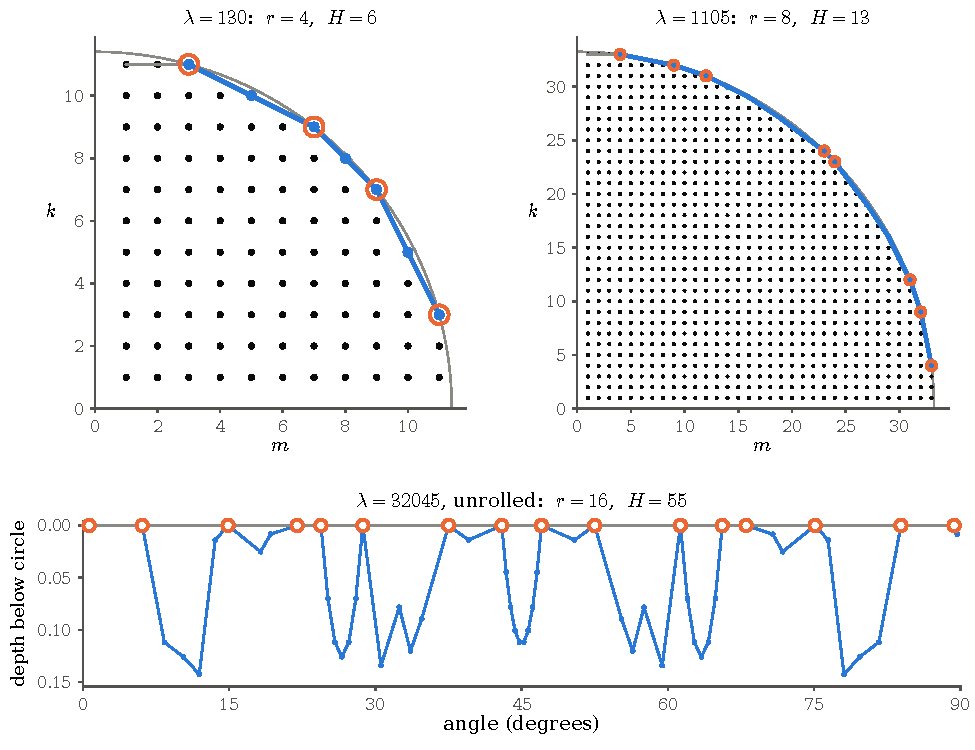
\includegraphics[width=0.96\textwidth]{fig_hull.pdf}
\caption{Top: the set $S'(\lambda)$ (dots), the circle $m^2+k^2=\lambda$, and the upper chain
of $\conv S'(\lambda)$. The slanted primitive segments (blue, with their endpoints marked) are
the ones counted by $H(\lambda)$, and the $r(\lambda)$ lattice points on the circle are
circled. At both levels $\lceil H/2\rceil=r-1$, so Theorem~C applies with equality. Bottom:
the lattice points of the upper chain at $\lambda=32045$, plotted by their angle and their
distance below the circle. Between two neighbouring points on the circle the hull dips inside
and picks up extra segments. Here $H=55$, against $2r-3=29$.}
\label{fig:hull}
\end{figure}

%=====================================================================================
\section{\texorpdfstring{The extended Courant property up to $\SweepX$ and for large $\lambda$}{The extended Courant property up to 10\textasciicircum 9 and for large lambda}}
\label{sec:computation}

By Theorem~C, ECP at $\lambda$ follows from the inequality $H(\lambda)\ge2r(\lambda)-3$, which
only involves lattice points. In this section we check this inequality by computer up to
$\SweepX$, and then we use the theorem of Balog and B\'ar\'any to prove it for all large
$\lambda$.

\subsection{The computation}
\begin{theorem}[Theorem D(i)]\label{thm:computation}
$H(\lambda)\ge2r(\lambda)-3$ for every eigenvalue $\lambda\le\SweepX$ of the square. Hence
the square has the extended Courant property at every $\lambda\le\SweepX$.
\end{theorem}

\begin{proof}[Proof (computer-assisted)]
For each $\lambda\le\SweepX$ with $r(\lambda)\ge1$ we computed $H(\lambda)$ exactly: the
column heights $c(m)=\max\{k:m^2+k^2\le\lambda\}$, $1\le m\le\lfloor\sqrt{\lambda-1}\rfloor$,
the upper convex hull of the points $(m,c(m))$ by a monotone chain, and the sum of
$\gcd(|\Delta m|,|\Delta k|)$ over the hull edges with $\Delta m\ne0\ne\Delta k$. Only integer
arithmetic is used. The computation was done by two programs that share no code, and which
differ in how they compute $r(\lambda)$ (direct counting of representations versus the
factorisation formula $r(\lambda)=\prod_{p\equiv1\,(4)}(e_p+1)-[\lambda=\square]$ when all
exponents $e_p$ of primes $p\equiv3\pmod 4$ are even, and $r(\lambda)=0$ otherwise), in how they
compute the column heights (integer square roots versus a monotone pointer), and in the
direction in which the hull is built. Both report no failures, and their per-decade statistics
agree exactly. They also agree with the Python reference implementation and with the exact
dynamic programme for $LB(\lambda)$ wherever these were run (Appendix~\ref{app:code}).
\end{proof}

Table~\ref{tab:slack} records the minimum of the slack $\lceil H/2\rceil-(r-1)$ per decade.
The slack is zero exactly at $\lambda\in\{2,5,8,10,13,20,25,34,50,65,73,85,130,205,221,425,650,
725,925,1105,2465\}$ and positive for all other eigenvalues up to $\SweepX$. Moreover, it is at least
$6$ above $10^4$, at least $169$ above $10^7$, and at least $475$ above $10^8$.

\begin{table}[t]
\centering
\begin{tabular}{lrrr}
\toprule
range & eigenvalues & min slack & attained at\\
\midrule
$[1,10^2)$ & 34 & 0 & 2, 10, \dots\\
$[10^2,10^3)$ & 274 & 0 & 130, \dots\\
$[10^3,10^4)$ & 2\,382 & 0 & 1105, 2465\\
$[10^4,10^5)$ & 21\,183 & 6 & 18\,850\\
$[10^5,10^6)$ & 192\,034 & 24 & 107\,185\\
$[10^6,10^7)$ & 1\,768\,321 & 66 & 1\,204\,450\\
$[10^7,10^8)$ & 16\,470\,067 & 169 & 10\,062\,130\\
$[10^8,10^9]$ & 154\,764\,314 & 475 & 100\,325\,125\\
\bottomrule
\end{tabular}
\medskip
\caption{Minimum of $\lceil H(\lambda)/2\rceil-(r(\lambda)-1)$ over the eigenvalues in each range.
ECP holds wherever this is non-negative.}
\label{tab:slack}
\end{table}

\subsection{\texorpdfstring{Large $\lambda$}{Large lambda}}
Let $V(R)$ be the number of vertices of the convex hull of $\Z^2\cap\{|z|\le R\}$. Balog and
B\'ar\'any \cite[Theorem~1]{BalogBarany} proved that $V(R)$ has order exactly $R^{2/3}$: there
are absolute constants $c_1,c_2>0$ such that $c_1R^{2/3}\le V(R)\le c_2R^{2/3}$ for all large
enough $R$, say $R\ge R_0$; their proof gives $c_1\approx0.33$ and $c_2\approx5.54$, but no explicit value of
``large enough''. See also \cite[(1.1) and Theorem~1]{BaranyLarman}, where this is restated and
extended to balls in every dimension.

\begin{lemma}\label{lem:HV}
$H(\lambda)\ge V(\sqrt\lambda)/4-4$ for every $\lambda\ge5$.
\end{lemma}

\begin{proof}
Let $K$ be the convex hull of $\Z^2\cap\{|z|\le\sqrt\lambda\}$ and $Q=\conv S'(\lambda)$. The
boundary of $Q$ consists of an edge on the line $m=1$, an edge on the line $k=1$, and the upper
chain; the only vertex of $Q$ not on the upper chain (including its endpoints) is $(1,1)$. A vertex of
$K$ in the open first quadrant lies in $S'(\lambda)$ and is extreme in $K\supseteq Q$, hence a
vertex of $Q$. It is not $(1,1)$, because for $\lambda\ge5$ the point $(1,1)$ lies inside the
segment from $(1,-2)$ to $(1,2)$. The set $\Z^2\cap\{|z|\le\sqrt\lambda\}$ is invariant
under rotation by $\pi/2$, which permutes the four open quadrants, and at most four vertices of
$K$ lie on the axes. Thus at least $(V-4)/4$ vertices of $K$ lie in the open first quadrant, and
the upper chain of $Q$ has at least that many vertices. It therefore has at least $(V-4)/4-1$
edges, of which at most two (a horizontal first edge and a vertical last edge) are
axis-parallel. Each slanted edge contains at least one primitive segment, so
$H(\lambda)\ge(V-4)/4-3=V/4-4$.
\end{proof}

\begin{figure}[t]
\centering
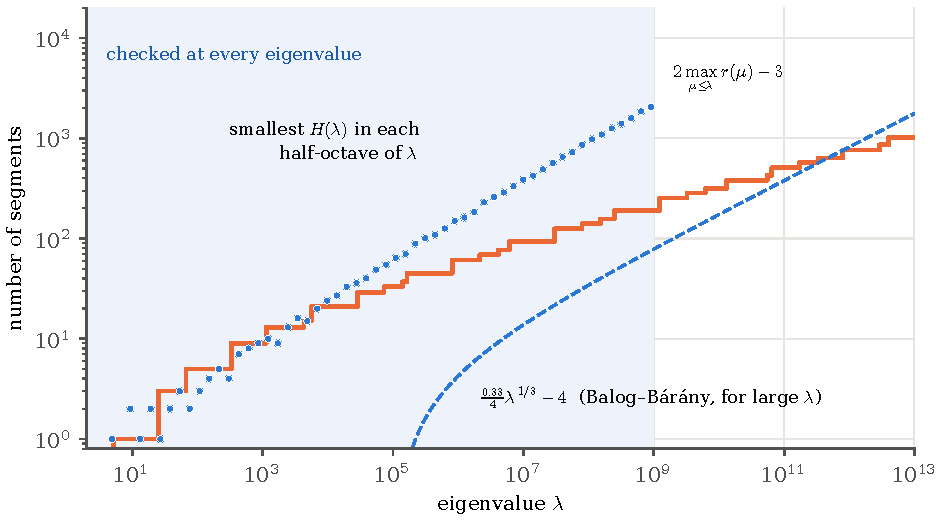
\includegraphics[width=0.86\textwidth]{fig_supply.pdf}
\caption{Theorem~D in one picture. Dots: the smallest value of $H(\lambda)$ among the
eigenvalues with $r(\lambda)\ge2$ in each window $[2^{j/2},2^{(j+1)/2})$, up to $\SweepX$.
Staircase: $2\max_{\mu\le\lambda}r(\mu)-3$, the largest right-hand side of the criterion
$H\ge2r-3$ that occurs up to $\lambda$. Dashed: the lower bound for $H(\lambda)$ that follows
from Lemma~\ref{lem:HV} and the theorem of Balog and B\'ar\'any, which is valid only for large
$\lambda$. In the shaded range the criterion is checked level by level
(Theorem~\ref{thm:computation}); below about $10^4$ some dots lie under the staircase, because
the two extremes are attained at different levels. The dashed curve stays above the staircase
only beyond about $10^{12}$ (Remark~\ref{rem:gap}).}
\label{fig:supply}
\end{figure}

\begin{theorem}[Theorem D(ii)]\label{thm:large}
There is an absolute constant $\lambda_0$ such that the square has the extended Courant
property at every $\lambda\ge\lambda_0$.
\end{theorem}

\begin{proof}
The positive solutions of $m^2+k^2=\lambda$ are at most a quarter of all integer solutions, so
by Jacobi's formula $r(\lambda)\le\sum_{d\mid\lambda}\chi_{-4}(d)\le\tau(\lambda)$, the number of
divisors of $\lambda$, and $\tau(\lambda)\le C_\epsilon\lambda^{\epsilon}$ for every
$\epsilon>0$. By Lemma~\ref{lem:HV} and the theorem of Balog and B\'ar\'any,
$H(\lambda)\ge\tfrac{c_1}{4}\lambda^{1/3}-4$ for $\lambda\ge\max(5,R_0^2)$. Taking $\epsilon=1/4$, we
get $H(\lambda)\ge2r(\lambda)-3$ for all sufficiently large $\lambda$, and
Theorem~\ref{thm:hull} applies.
\end{proof}

\begin{remark}[The remaining gap]\label{rem:gap}
Theorems~\ref{thm:computation} and~\ref{thm:large} leave open only the levels in
$(\SweepX,\lambda_0)$. Any explicit lower bound of the form $H(\lambda)\ge c\lambda^{1/3}-C$,
combined with the explicit records of $r(\lambda)$ (for instance $r(\lambda)\le72$ for
$\lambda\le10^8$ and $r(\lambda)\le384$ for $\lambda\le10^{12}$), turns the remaining gap into a
finite computation. Numerically $H(\lambda)/\lambda^{1/3}$ is at least $0.78$ on $[10^3,10^4)$,
at least $1.16$ on $[10^4,10^5)$, at least $1.80$ on $[10^7,10^8)$ and at least $2.07$ on
$[10^8,10^9)$, increasing slowly, while the slack in Table~\ref{tab:slack} grows quickly
(Figure~\ref{fig:supply}). Comparing with the records of $r(\lambda)$, a bound with $c=1/4$ and
$C=4$, valid for all $\lambda>\SweepX$, would already finish the proof with no further
computation: the last level at which $\tfrac14\lambda^{1/3}-4<2r(\lambda)-3$ is possible lies
below $5\times10^8$. The constant $c_1\approx0.33$ of Balog and B\'ar\'any gives only
$c\approx0.08$ through Lemma~\ref{lem:HV}. This would require checking up to about
$8\times10^{11}$ (the bound first stays above $2r(\lambda)-3$ after the record
$r(785\,817\,263\,725)=384$), and it would also need an explicit value of their threshold for
``large enough''.
\end{remark}

\begin{remark}[Vertices and segments]\label{rem:segments}
Two numerical observations explain why the criterion has so much room. First, the number of
vertices of the upper chain of $\conv S'(\lambda)$ concentrates around $0.87\,\lambda^{1/3}$
(the median over samples of $300$ eigenvalues is $0.88$ near $10^5$ and $0.87$ near $10^9$).
This agrees with the theorem of Balog and Deshouillers \cite{BalogDeshouillers} that the
average of $V(R)/R^{2/3}$ over $R$ tends to a constant close to $3.453$, since
$3.453/4\approx0.863$. Second, a slanted edge of the hull usually contains more than one
primitive segment, and this number increases throughout the range of our computation: its
median is about $2.0$ near $10^3$, $2.6$ near $10^5$, $2.9$ near $3\times10^6$ and $3.4$ near
$10^9$. So $H(\lambda)$ is several times larger than the number of vertices, and
Lemma~\ref{lem:HV}, which only counts vertices, loses this factor. A heuristic count of the
lattice points on the outermost lattice lines in each direction suggests that
$H(\lambda)/\lambda^{1/3}$ is bounded and has a mean value, approached slowly, with an error of
relative size about $\lambda^{-1/12}$. We do not pursue this here.
\end{remark}

%=====================================================================================
\section{Exact values and sharpness}\label{sec:sharp}

It is natural to ask how good the bound $U(\lambda)$ is. In this section we look at small levels,
where we can compute $U(\lambda)$ exactly and compare it with explicit examples.

For $\lambda\le130$ we computed $U(\lambda)$ exactly by exhausting all admissible multisets
(Appendix~\ref{app:code}). Table~\ref{tab:U} lists the result. In this range
$U(\lambda)\le\kappa(\lambda)$, with equality exactly at
$\lambda\in\{5,8,10,13,20,25,34,50,65,85,130\}$.

\begin{table}[t]
\centering\small
\begin{tabular}{rrrrrr@{\qquad}rrrrrr}
\toprule
$\lambda$&$r$&$N$&$\kappa$&$U$&$\lceil H/2\rceil$&$\lambda$&$r$&$N$&$\kappa$&$U$&$\lceil H/2\rceil$\\
\midrule
5&2&3&2&\textbf{2}&1&72&1&48&48&46&2\\
8&1&4&4&\textbf{4}&0&73&2&50&49&48&1\\
10&2&6&5&\textbf{5}&1&74&2&52&51&49&2\\
13&2&8&7&\textbf{7}&1&80&2&54&53&52&2\\
17&2&10&9&8&2&82&2&56&55&53&3\\
18&1&11&11&9&1&85&4&60&57&\textbf{57}&3\\
20&2&13&12&\textbf{12}&1&89&2&62&61&59&3\\
25&2&15&14&\textbf{14}&1&90&2&64&63&61&3\\
26&2&17&16&15&2&97&2&66&65&63&3\\
29&2&19&18&17&2&98&1&67&67&65&1\\
32&1&20&20&18&1&100&2&69&68&66&2\\
34&2&22&21&\textbf{21}&1&101&2&71&70&67&3\\
37&2&24&23&21&2&104&2&73&72&70&3\\
40&2&26&25&24&2&106&2&75&74&72&3\\
41&2&28&27&26&2&109&2&77&76&73&3\\
45&2&30&29&28&2&113&2&79&78&76&3\\
50&3&33&31&\textbf{31}&2&116&2&81&80&79&2\\
52&2&35&34&33&2&117&2&83&82&80&3\\
53&2&37&36&34&2&122&2&85&84&81&4\\
58&2&39&38&37&2&125&4&89&86&85&4\\
61&2&41&40&39&2&128&1&90&90&87&2\\
65&4&45&42&\textbf{42}&3&130&4&94&91&\textbf{91}&3\\
68&2&47&46&44&3&&&&&&\\
\bottomrule
\end{tabular}
\medskip
\caption{Exact values of $U(\lambda)$ at all eigenvalues $5\le\lambda\le130$, with $N=\dim E_\lambda$, the multiplicity $r$, and the lower bound $\lceil H/2\rceil$ for $N-U$ from Theorem~\ref{thm:hull}. Bold: $U=\kappa$. In this range $N-U=LB(\lambda)$ exactly.}
\label{tab:U}
\end{table}


\begin{proposition}\label{prop:sharp}
At $\lambda=5,8,10,13,20,25,34$ the maximal number of nodal domains of a combination in
$E_\lambda$ equals $\kappa(\lambda)$, namely $2,4,5,7,12,14,21$.
\end{proposition}

\begin{proof}
The upper bound is Table~\ref{tab:U}. For the lower bound, the polynomials
\[
X,\quad XY,\quad X^2+Y^2-\tfrac32,\quad XY(X+Y-\tfrac12),\quad
(X-\tfrac{17}{20})(Y-\tfrac{17}{20})(X^2+Y^2-\tfrac32),
\]
\[
(X^2-\tfrac{9}{100})(Y^2-\tfrac{9}{100})(Y-X-\tfrac1{10}),\quad
(X^2-\tfrac{289}{400})(Y^2-\tfrac{289}{400})(X^2+Y^2-\tfrac32)
\]
have supports in $S(\lambda)$ for the respective $\lambda$. Each is a product of distinct lines and at most one circle, none containing a side of $B$, and
every point of $B$ where two of these curves meet is a transversal crossing of exactly two of
them. So Lemma~\ref{lem:euler} gives $\nu_B=1+\varepsilon/2+\#\{\text{crossings in }B\}$.
For example, at $\lambda=34$ the four lines and the circle of radius $\sqrt{3/2}$ have
$\varepsilon=8+8$ ends and $4+8$ crossings, so $\nu_B=1+8+12=21$. The other cases are similar.
(We have also confirmed them by grid counts at three resolutions.)
\end{proof}

\begin{proposition}\label{prop:17-18}
The maximal number of nodal domains of a combination in $E_{17}$ is $8$, and in $E_{18}$ it
is $9$. Here $\kappa(17)=9$ and $\kappa(18)=11$.
\end{proposition}

\begin{proof}
$U(17)=8$ and $U(18)=9$ (Table~\ref{tab:U}). The polynomials $(X^2+Y^2-\tfrac32)(Y-X)$ and
$(X^2-\tfrac9{25})(Y^2-\tfrac9{25})$ have supports in $S(17)$ and $S(18)$ respectively (note that
$S(17)$ is the set of exponents of total degree at most $3$, and $S(18)=S(17)\cup\{(2,2)\}$),
and have $1+5+2=8$ and $1+4+4=9$ nodal domains by Lemma~\ref{lem:euler}.
\end{proof}

\begin{remark}[Comparison with the literature]
In his thesis, Zhu \cite[\S4.4.1]{ZhuThesis} examines the square case by case for the first
$n\le14$ eigenfunctions. For $n=11$ (that is, $\lambda=18$) the thesis states that a combination
has ``at most ten'' nodal domains. This is an upper bound, consistent with $U(18)=9$, and
Proposition~\ref{prop:17-18} shows it is not attained. In particular, the configuration drawn there with ten
domains, a line times a cubic, cannot be realised by a polynomial with exponents in $S(18)$. The entries $8$ for $n=9,10$ and $12$ for $n=12,13$ agree with $U(17)=8$ and
$U(20)=12$.

The corner cap is needed to determine the maximum at $\lambda=18$: without it the four side
restrictions, cubics in this case, could have $12$ roots instead of $10$, and the bound
would be $10$ instead of $9$. More importantly, without the cap a factor whose polygon is a
triangle $\conv\{0,ae_1,be_2\}$ with $\gcd(a,b)=1$ would cost nothing in the
identity~\eqref{eq:identity}, and
Theorem~\ref{thm:hull} would fail.
\end{remark}

At $\lambda=50,65,85,130$ we have $U(\lambda)=\kappa(\lambda)$, but we do not know whether
$\kappa$ is attained. At $\lambda=50$ the best construction we found has $28$ nodal domains,
against $\kappa(50)=31$.

%=====================================================================================
\section{Questions}\label{sec:questions}

We close with some questions that the results above leave open.

\begin{question}
Close the gap of Remark~\ref{rem:gap}: prove an explicit lower bound for the number of edges of
the convex hull of the lattice points in a quarter disc that, together with the computation of
Theorem~\ref{thm:computation} (perhaps extended), gives ECP for the square at every level.
\end{question}

\begin{question}
Does $H(\lambda)/\lambda^{1/3}$ have a mean value, in the sense of Balog and Deshouillers
\cite{BalogDeshouillers} for the number of vertices, and what is it
(Remark~\ref{rem:segments})? Since $r(\lambda)\le C\lambda^{1/6}$ with an explicit constant
$C$, even an explicit bound $H(\lambda)\ge2C\lambda^{1/6}$ for $\lambda>\SweepX$ would close
the gap.
\end{question}

\begin{question}
Is $U(\lambda)$ the true maximum of $\nu$ on $E_\lambda$? In particular, is $\kappa(\lambda)$
attained at $\lambda=50,65,85,130$?
\end{question}

\begin{question}
The method uses only the structure of $E_\lambda$ as a space of polynomials with exponents in a
down-closed set. For a rectangle $(0,\pi)\times(0,\pi/\alpha)$ the eigenfunctions have the same
form with $S(\lambda)$ replaced by the lattice points under an ellipse. Does the analogue of
Theorem~C hold, and does it prove the conjecture of Gladwell and Zhu for rectangles? Similar
questions arise for other domains whose eigenfunctions are polynomial in suitable coordinates,
such as the equilateral triangle and the hemisphere.
\end{question}

%=====================================================================================
\appendix
\section{Computations and formal verification}\label{app:code}

The companion repository \cite{repo} contains the code and logs for everything below, with
instructions for rerunning it.

\subsection*{\texorpdfstring{Exact evaluation of $U(\lambda)$}{Exact evaluation of U}}
The values in Table~\ref{tab:U} are computed by a depth-first search over multisets of
polygons in $\mathcal D_\lambda$. Two facts make the search exact.
\begin{enumerate}[label=(\alph*),nosep]
\item \emph{The list of polygons is complete.} A down-closed $D\in\mathcal D_\lambda$ is the
convex hull of the lattice points under a non-increasing column profile
$c_0\ge c_1\ge\dots\ge c_{w_x}\ge0$, and conversely. The program enumerates all such profiles
with entries at most $\max_{\Delta_\lambda}y$, forms the hull, keeps it if all its vertices lie in
$S(\lambda)$ (equivalently, the hull lies in the convex set $\Delta_\lambda$), and discards
points and long axis segments.
\item \emph{The search is exhaustive.} Multisets are visited as non-decreasing index sequences.
A branch is pruned only when the partial Minkowski sum $A$ leaves $\Delta_\lambda$, and then no
extension fits, because every polygon contains $0$ and so $A\subseteq A+D$. The objective is
computed incrementally using $\sum_{j<i}\MV(D_j,D_i)=\MV(D_1+\dots+D_{i-1},D_i)$, and the last
term of \eqref{eq:Umulti} depends only on the multiset of values $\eta(D_i)$, so memoising on
(next index, partial sum, multiset of $\eta$'s) is exact. The maximum over $T$ is attained, for
each $|T|=j$, by the $j$ largest values of $\eta$.
\end{enumerate}
All arithmetic is in integers (Pick's formula, doubled areas, gcds). A second implementation,
written independently by a colleague from the text of the proof alone, without access to our
code, reproduces all $45$ values for $5\le\lambda\le130$.

\subsection*{\texorpdfstring{The dynamic programme for $LB(\lambda)$}{The dynamic programme for LB}}
A nonempty down-closed lattice polygon $D\subseteq\Delta_\lambda$ is determined by its right
column $x_0$, the height $y_0$ of its right side, and the remaining edges $k_j(-a_j,b_j)$ of its
upper chain, with $(a_j,b_j)$ primitive, $a_j\ge1$, $b_j\ge0$, slopes $b_j/a_j$ strictly
decreasing, and the chain ending on the $y$-axis. It lies in $\Delta_\lambda$ if and only if its
vertices lie in $S(\lambda)$. The programme keeps states (vertex, parity vector in $(\Z/2)^3$),
processes the primitive directions in order of decreasing slope, and extends every state by
$k=1,2,\dots$ copies of the current direction while the endpoint stays in $S(\lambda)$. The cost
$\miss(D)+(n(D)+\varphi(o(D)))/2$ is additive along the chain (columns are charged once each,
slanted edges add their lattice length, and the parity vector records the classes), so the
minimum over states equals $LB(\lambda)$. The programme agrees with a brute-force minimum over
all down-closed polygons at all $68$ eigenvalues $\lambda\le200$, satisfies $LB=N-U$ at all $45$
eigenvalues $5\le\lambda\le130$, gives $LB(\lambda)\ge r(\lambda)-1$ at all $1401$ eigenvalues
$\lambda\le5000$, and satisfies $LB(\lambda)\ge\lceil H(\lambda)/2\rceil$ throughout, with
$LB-\lceil H/2\rceil\le1$ there. The colleague's implementation agrees on all $1401$
values.

\subsection*{The sweep of Theorem~\ref{thm:computation}}
The two programs described in the proof of Theorem~\ref{thm:computation} are written in C. They
agree on $H(\lambda)$ and $r(\lambda)$ at every one of $10\,599$ spot-checked levels and on all
per-decade statistics up to $\SweepX$.

\subsection*{Lean}
Lemma~\ref{lem:roots} is formalised in Lean~4 with Mathlib as
\texttt{card\_roots\_Ioo\_add\_le}: for a nonzero real polynomial $p$, the number of roots in
$(-1,1)$ counted with multiplicity, plus one for each sign mismatch at $\pm1$, is at most
$\deg p$. The file also proves the cubic case of the corner cap used at $\lambda=17,18$
(\texttt{ends\_cap\_cubic}: four side cubics with shared leading coefficients on opposite sides
and consistent nonzero corner values have at most $10$ roots on the open sides). There is no
\texttt{sorry}, and \texttt{\#print axioms} reports only \texttt{propext},
\texttt{Classical.choice} and \texttt{Quot.sound}.

\subsection*{Numerical evidence}
Grid counts of nodal domains are used only to double-check the explicit constructions of
Section~\ref{sec:sharp}, never in a proof.

\section*{Acknowledgements}
The author thanks Professor Eugenia Malinnikova, the author's mentor and adviser, for
guidance, and a colleague, who prefers to remain anonymous, for independently
reimplementing the computation of $U(\lambda)$ and $LB(\lambda)$ from the written proof.

\subsection*{Use of AI tools}
Generative AI tools (Anthropic's Claude) were used throughout this work, building on the
author's earlier report \cite{Sanayei21}: to repair and complete parts of the proofs, to write
the programs and the Lean formalisation, to prepare the figures, and to review and edit the
text.

\bibliographystyle{amsplain}
\bibliography{refs}

\end{document}
